\begin{frame}{Sur les réseaux sociaux, une relation avant tout parasociale}
    \textbf{Relation parasociale} = phénomène par lequel une personne développe un sentiment d'intimité avec une figure médiatique ou fictive qui n'a pourtant pas vraiment conscience de son existence.\\
    Sur les réseaux sociaux, le rôle du \textit{community management}: repose sur l'exploitation de cette relation parasociale, en jouant sur le registre de l'intime.\\


\end{frame}

\begin{frame}{Un rôle actif dans la visibilité}
    Qu'est-ce que ça change pour le lecteur comme cible éditoriale ?\\
    Moins le lecteur s'attarde sur des profils, moins ils vont apparaître en priorité sur le fil d'actualité\\

    Autre type de relation entre l'écrivain et le lecteur: le patron-mécène\\
\end{frame}
\begin{frame}{Le \textit{buisiness model} du financement participatif \textit{crowdfunding}}
    \centering
\begin{minipage}{0.45\textwidth}
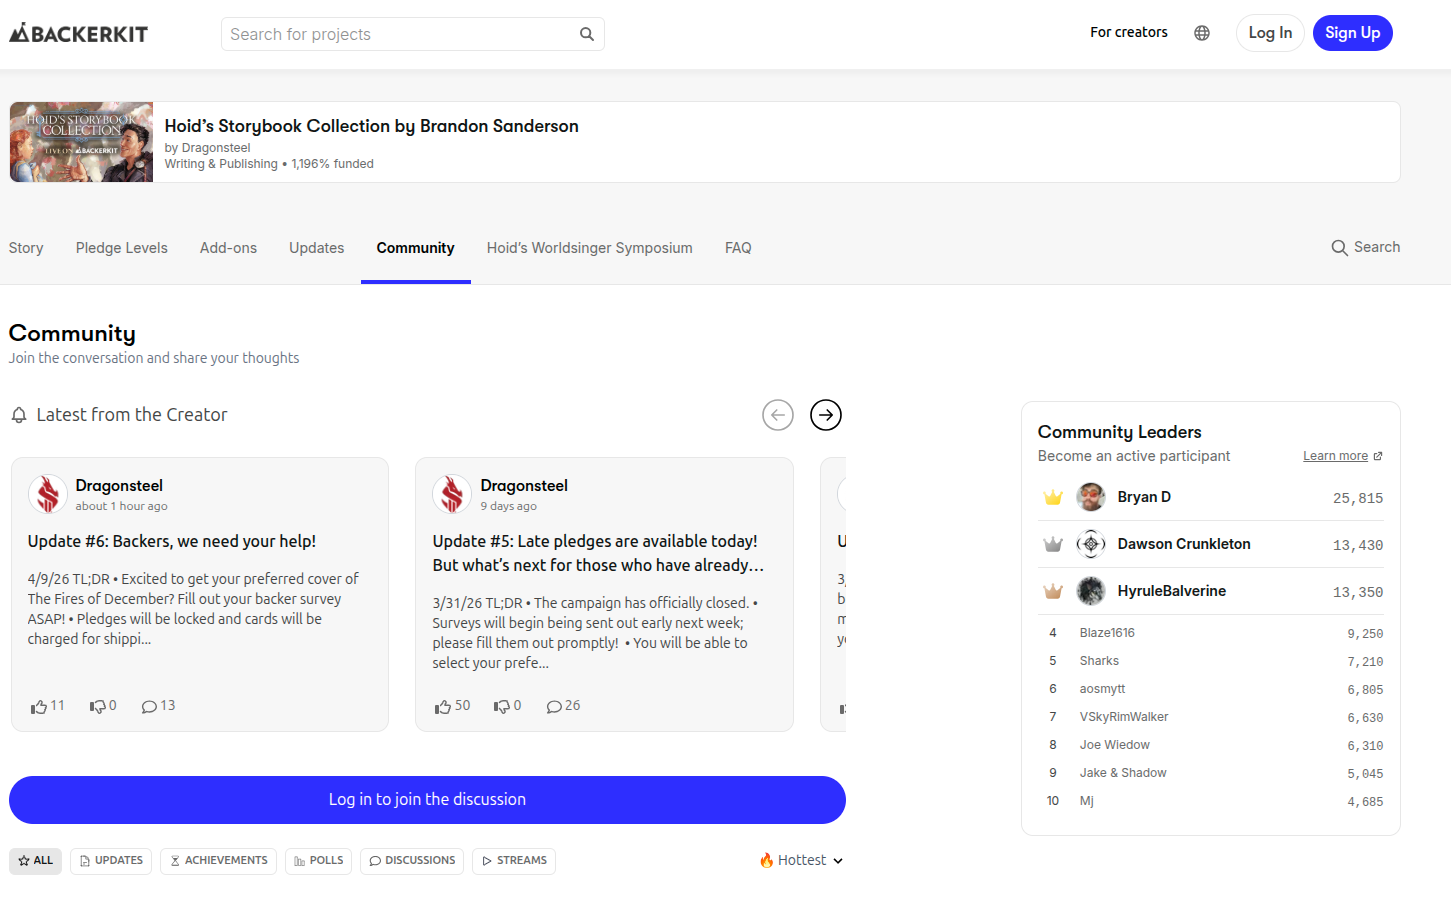
\includegraphics[width=\textwidth]{Images/crowfounding_sanderson.png}
\end{minipage}\hfill
\begin{minipage}{0.45\textwidth}
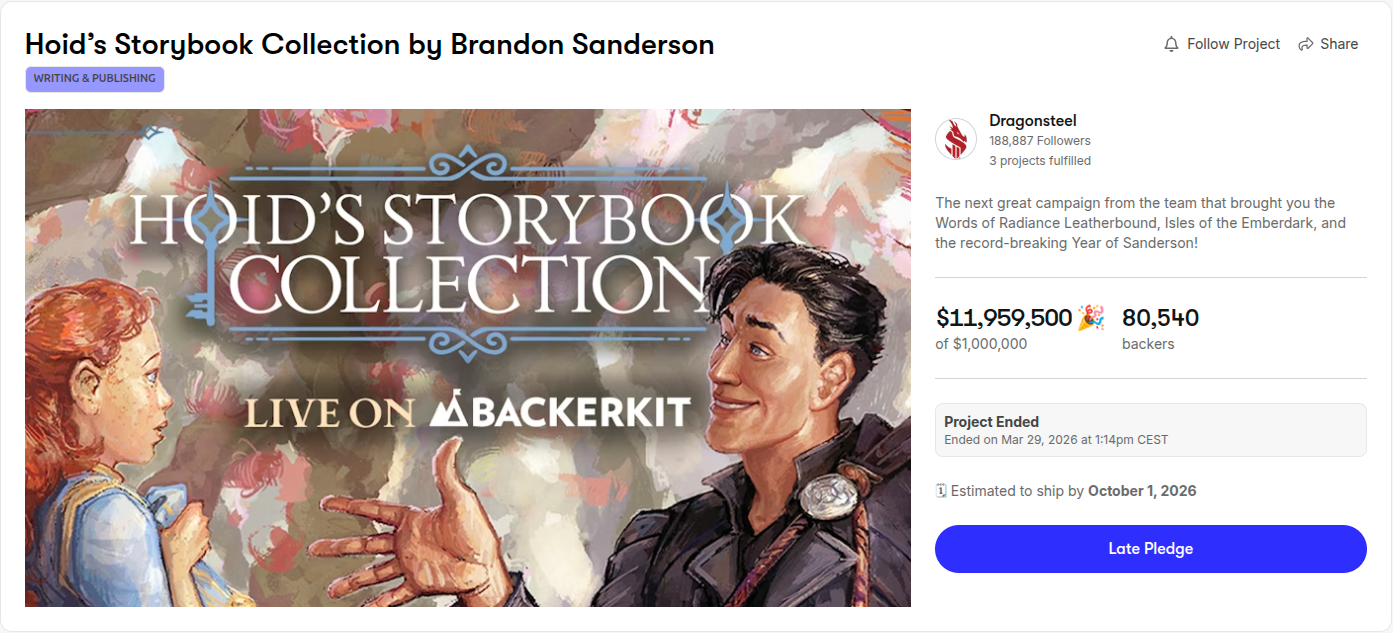
\includegraphics[width=\textwidth]{Images/crowfounding_sanderson2.png}
\end{minipage}\par
\vskip\floatsep% normal separation between figures
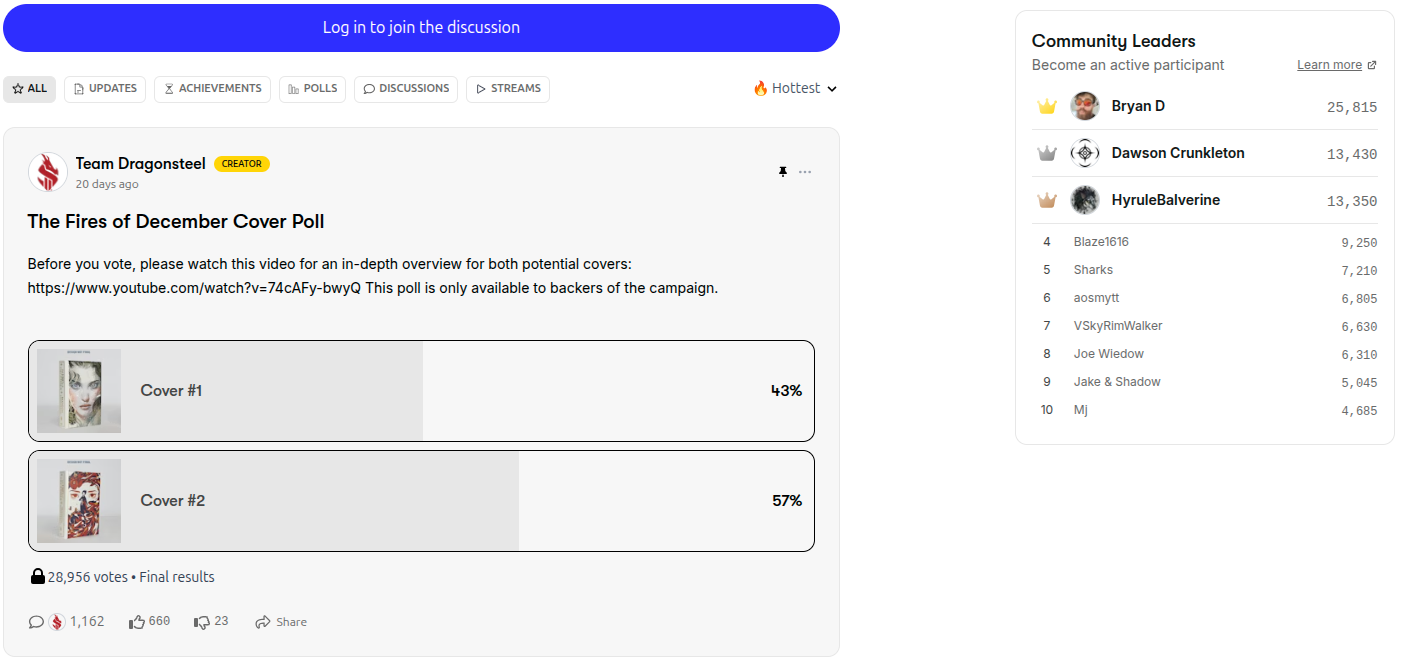
\includegraphics[width=0.45\textwidth]{Images/communauté_sanderson.png}
\end{frame}


\begin{frame}{Le paradigme du "patron" (Mécène)}
    \textbf{Patreon: une sorte de contre-culture participative (Servanne Monjour)?}\\  
    Là où normalement on veut le plus d'attention possible, Patreon propose l'inverse: une communauté fermée (payante) mais avec des intéractions plus proches avec l'auteur.rice.\\
    \vspace{1em}
    \textbf{L'impératif participatif (Marta Severo)} = permettre la participation n'est plus seulement un moyen de gagner de l'audience, c'est aussi un moyen de gagner en légitimité. 
    \textrightarrow{} Mais la participation, du fait de la plateformisation croissante, est de plus en plus régulée.
\end{frame}

\begin{frame}{Le paradigme du "patron" (Mécène)}
    \begin{center}
        {\small \textit{Nota 2 : c'est aussi le soutien que représente à mes activités cet espace \#Patreon qui m'a permis de désactiver le plus totalement possible les publicités parasites sur ma chaîne YouTube, désormais le poumon respirant du site. Pour cela aussi, merci.}}\\
        \textbf{François Bon}
    \end{center}
\end{frame}

\begin{frame}{Le paradigme du "patron" (Mécène)}
    La plupart des plateformes créatives et de financement participatif jouent sur la monétisation de la relation parasociale qui se crée entre le créateur et sa communauté, à partir d'une mise en scène de l'intime, Patréon joue sur la carte de la professionnalisation, et valorise un discours du travail.\\
    Rappelle un peu les salons littéraires.
    
\end{frame}
